\documentclass[]{../template/Report}%方括号内写yuxi即生成预习报告\documentclass[yuxi]{../template/Report}
\settemplatedir{../template/}%设置模板路径

\exname{非平衡电桥} %实验名称
\extable{2} %实验桌号
\instructor{居乐乐} %指导教师
\class{信工2401} %班级
\name{姚舜瑜} %姓名
\stuid{3240100532} %学号

\nyear{2025} %年
\nmonth{9} %月
\nday{30} %日
\nweekday{二} %星期几,e.g. \nweekday{三}
\daypart{上午}%上午/下午

\redate{} %如有实验补做,补做日期
\resitu{} %情况说明:

\begin{document}
\maketitle%输出封面

\section{预习报告(10分)}
\subsection{实验综述(5分)}

\subsubsection{实验目的}
\begin{enumerate}
	\item 掌握非平衡电桥的工作原理与测量方法,熟悉电桥电路的调节与读数流程;
	\item 应用非平衡电桥测量金属材料的电阻随温度变化的特性,并计算材料的电阻温度系数。
\end{enumerate}

\subsubsection{实验原理}
非平衡电桥的主要作用是将因外界物理量(如压力、温度、应变等)变化引起的电阻变化,转换为易于测量的电压输出,从而实现对连续变化物理量的测量、监测与控制。
其在测量中具有高灵敏度和良好的线性响应特性,适用于精密测量和控制系统。其典型电路为四臂电桥,中点之间的电压差$U$为输出量,如下图:
\begin{figure}[H]
    \centering
    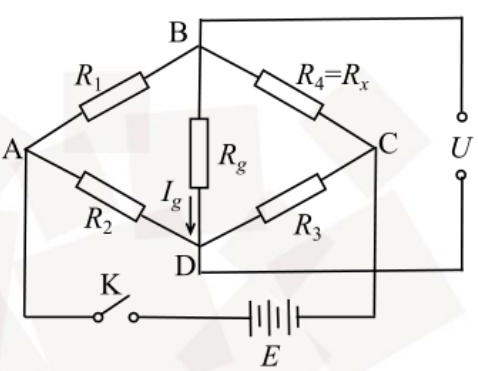
\includegraphics[width=0.4\textwidth]{figure/非平衡电桥示意图.png}
    \caption{非平衡电桥示意图}
    \label{fig:fig1}
    % 实验条件:E = 1.3 V;理论值 alpha_theory = 0.004218
\end{figure}
\noindent 设四臂电阻分别为 $R_1,R_2,R_3,R_x$($R_x$ 为被测电阻),则两中点电位为:
\begin{equation}
\begin{aligned}
V_A&=\frac{R_2}{R_1+R_2}E\\
V_B&=\frac{R_x}{R_3+R_x}E
\end{aligned}
\end{equation}
因此输出电压为:
\begin{equation}
U=V_{\text{out}}=V_A-V_B
=\Big(\frac{R_2}{R_1+R_2}-\frac{R_x}{R_3+R_x}\Big)E.
\end{equation}
当被测量为温度时,金属在室温附近常可用线性温阻关系近似描述:
\begin{equation}
R_t=R_0(1+\alpha t),
\end{equation}
其中 $R_0$ 为参考温度(通常取 $0^{\circ}\mathrm{C}$ 或测量起始温度)时的电阻,$t$ 为相对于参考温度的温差(单位为 $^{\circ}\mathrm{C}$ 或 K),$\alpha$ 为电阻温度系数(单位 $\mathrm{K}^{-1}$)。当温度变化较小时($|\alpha t|\ll1$),线性近似成立,此时阻值增量可写为
\begin{equation}
    % 实验条件:E = 1.3 V;理论值 alpha_theory = 0.004218
\Delta R=R_t-R_0\approx R_0\alpha t.
\end{equation}
需要注意的是,金属阻值的精确温度依赖在不同温区可能不同:在室温及以上区间,电子——声子散射使阻值近似随温度线性增加;在低温区会出现明显的非线性,
但本实验在室温小范围内测量时采用线性近似足够精确,可用 $\Delta R\approx R_0\alpha t$ 来求解 $\alpha$。
在测量方案中,若将被测电阻置于电桥一臂并记为 $R_x$,为方便推导令 $R_x=R_1$ 并取对称条件
$R_1=R_2=R_3=R_0$。将这些代入不平衡电桥的输出表达式(记电源电压为 $E$):
\begin{equation}
U=\frac{R_2R_x+R_2\Delta R_x-R_1R_3}{(R_1+R_x+\Delta R_x)(R_2+R_3)}\,E,
\end{equation}
化简得到(代入对称条件并整理):
\begin{equation}
U=\frac{\alpha t}{4+2\alpha t}\,E.
\end{equation}
从该精确表达可解出温度系数 $\alpha$:
\begin{equation}
\alpha=\frac{4U}{t\,(E-2U)}.
\end{equation}

\subsubsection{实验内容}
本实验仪器主要由非平衡直流电桥和温控装置组成。主要实验内容有两个方面:

\begin{enumerate}
    \item \textbf{应用非平衡电桥测量铜电阻($Cu50$)的温度系数。}
    \begin{enumerate}[label=\roman*.]
        \item 将功能开关置于非平衡电压档;
        \item 连接电路,待测电阻 $0^{\circ}\mathrm{C}$ 时为 $50\Omega$,将 $R_1,R_2,R_3$ 均设置为 $50\Omega$;
        \item 在不同温度点(间隔约 $5^{\circ}\mathrm{C}$)测量非平衡电压 $U$,记录对应温度 $t$ 与 $U$;
        \item 根据公式 $\alpha=\dfrac{4U}{t(E-2U)}$ 计算温度系数 $\alpha$。
    \end{enumerate}

    \item \textbf{应用平衡电桥测绘铜电阻($Cu50$)温度特性曲线。}
    \begin{enumerate}[label=\roman*.]
        \item 将功能开关置于平衡“5V”档;
        \item 连接电路,设置 $R_1=R_2$(平衡桥配置);
        \item 在相同温度点(间隔约 $5^{\circ}\mathrm{C}$)测量电阻值或对应的平衡调节值,记录温度与电阻;
        \item 绘制 $R-T$ 曲线,分析线性范围,并使用最小二乘拟合求出 $\alpha$。
    \end{enumerate}
\end{enumerate}


\subsection{实验重点(3分)}
\begin{enumerate}
    \item 理解非平衡电桥的工作原理;
    \item 掌握电桥电路的调节与读数流程,确保测量准确;
    \item 熟悉温控装置的使用,保证温度的稳定性。
\end{enumerate}

\subsection{实验难点(2分)}
\begin{enumerate}
    \item 如何控制温度稳定并保持在设定值附近;
    \item 实验误差影响因素较多,如何消除误差影响;
\end{enumerate}

\begin{fullreportonly}
\section{原始数据(20分)}
\begin{figure}[H]
    \centering
    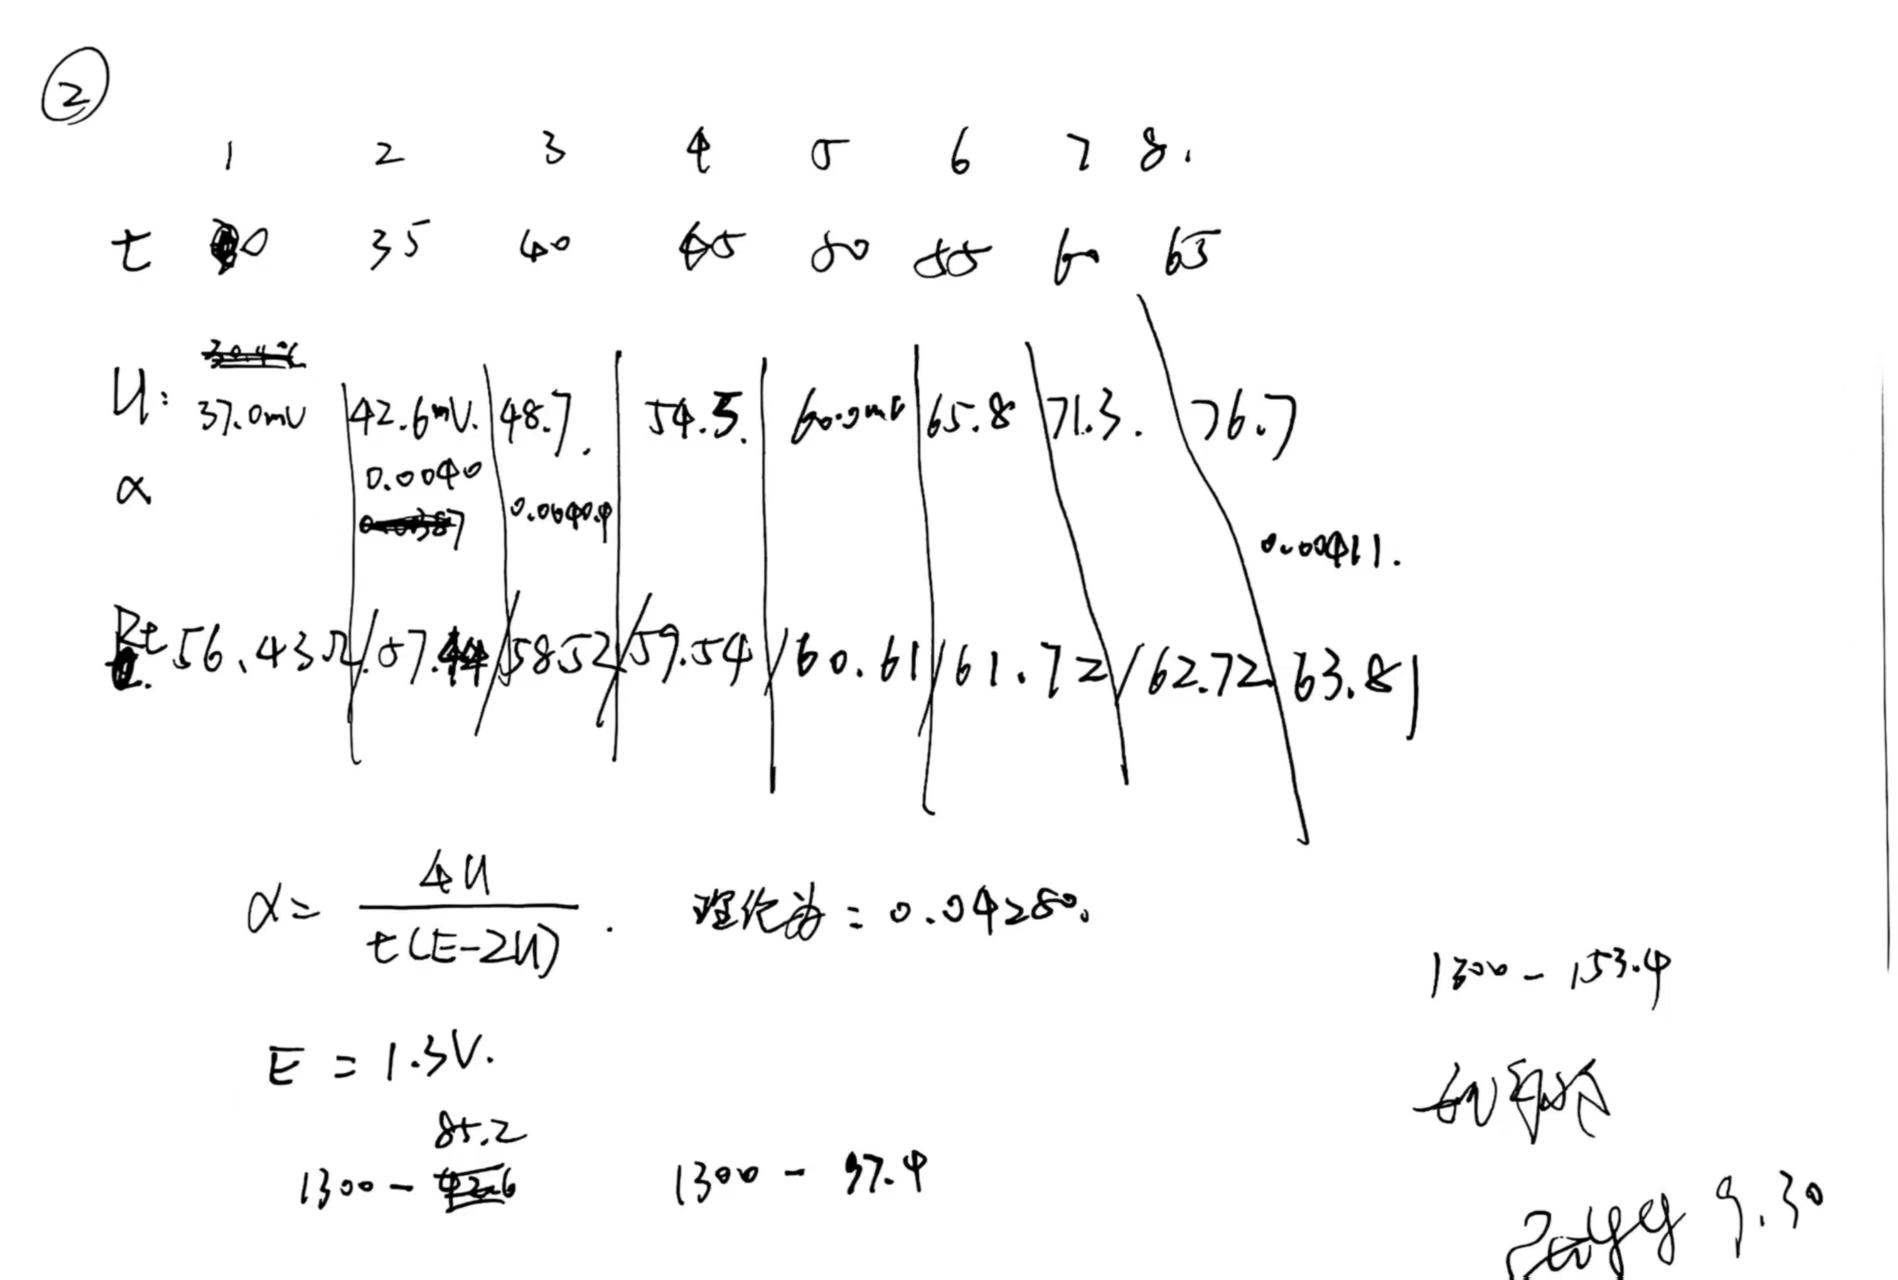
\includegraphics[width=0.8\textwidth]{figure/原始数据.jpg}
    \caption{原始数据记录图}
    \label{fig:fig2}
\end{figure}

\section{结果与分析(60分)}
\subsection{数据处理与结果(30分)}
\subsubsection{非平衡电桥测温度系数数据处理}
\begin{table}[H]
\centering
\caption{非平衡电桥测温度系数数据记录表}
\vspace{2mm}
{\small \centering 实验条件:E = 1.3\,V \quad; \quad $\alpha_{\mathrm{theory}}=0.004218$ \par}
\vspace{2mm}
\begin{tabularx}{0.9\textwidth}{>{\centering\arraybackslash}p{0.2\textwidth}|*{8}{>{\centering\arraybackslash}X}}
\hline
次序 & 1 & 2 & 3 & 4 & 5 & 6 & 7 & 8 \\
\hline
温度 $t/^{\circ}\mathrm{C}$ &30 &35 &40 &45 &50 &55 &60 &65 \\
\hline
不平衡电压 $U$/mV &37.0 &42.6 &48.7 &54.5 &60.0 &65.8 &71.3 &76.7 \\
\hline
计算 $\alpha$/$\left(10^{-3}\,^{\circ}\mathrm{C}^{-1}\right)$ & $4.025$ & $4.007$ & $4.050$ & $4.067$ & $4.068$ & $4.096$ & $4.106$ & $4.116$ \\
\hline
\end{tabularx}
\end{table}
由表可计算得到 8 个温度点的 $\alpha_i$,其平均值为 $\bar{\alpha}=4.0669\times10^{-3}\,^{\circ}\mathrm{C}^{-1}$

\subsubsection{平衡电桥测温度特性数据处理}
\begin{table}[H]
\centering
\caption{平衡电桥测温度特性数据记录表}
\vspace{2mm}
{\small \centering 实验条件:E = 1.3\,V \quad; \quad $\alpha_{\mathrm{theory}}=0.004218$ \par}
\vspace{2mm}
\begin{tabularx}{0.9\textwidth}{>{\centering\arraybackslash}p{0.2\textwidth}|*{8}{>{\centering\arraybackslash}X}}
\hline
次序 & 1 & 2 & 3 & 4 & 5 & 6 & 7 & 8 \\
\hline
温度 $t/^{\circ}\mathrm{C}$ &30 &35 &40 &45 &50 &55 &60 &65 \\
\hline
$R_t/\Omega$ &56.43 &57.44 &58.52 &59.54 &60.61 &61.72 &62.72 &63.81 \\
\hline
\end{tabularx}
\end{table}
根据上表的数据,对 $R_t$ 与 $t$ 进行最小二乘线性拟合:得到 $R(t)=a+bt$,其中 $a=50.06381\Omega$,$b=0.2112619\Omega/^{\circ}\mathrm{C}$,进而 $\alpha=\dfrac{b}{R_0}=4.219853\times10^{-3}\,^{\circ}\mathrm{C}^{-1}$。
\begin{figure}[H]
    \centering
    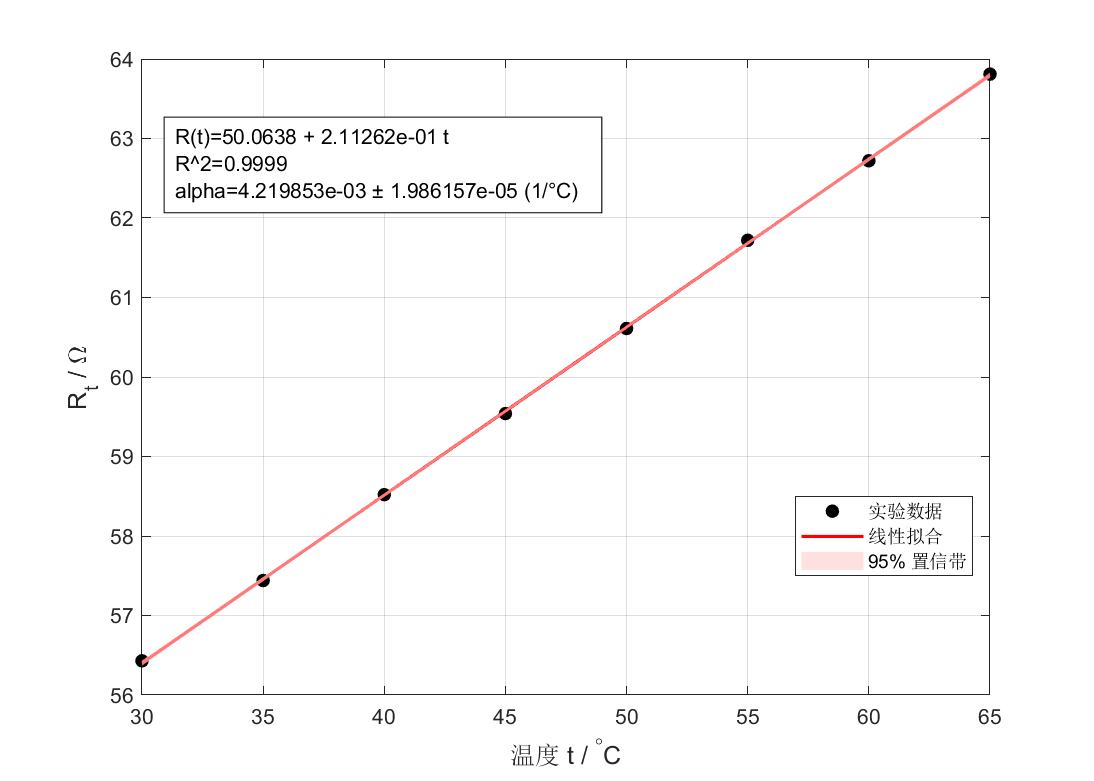
\includegraphics[width=0.6\textwidth]{figure/拟合.png}
    \caption{平衡电桥测温度特性拟合图}
    \label{fig:fig3}
\end{figure}


\subsection{误差分析(20分)}
\subsubsection{非平衡电桥测量的统计与不确定度}
对非平衡电桥所得 $\alpha_i$(单位 $10^{-3}\,^{\circ}\mathrm{C}^{-1}$):$4.025,\,4.007,\,4.050,\,4.067,\,4.068,\,4.096,\,4.106,\,4.116$,有:
\begin{equation}
\bar{\alpha}=4.0669\times10^{-3}\,^{\circ}\mathrm{C}^{-1},\qquad s=0.0386\times10^{-3}\,^{\circ}\mathrm{C}^{-1},\qquad u_A=\frac{s}{\sqrt{8}}=0.0136\times10^{-3}\,^{\circ}\mathrm{C}^{-1}.
\end{equation}

若忽略型 B 不确定度,取 A 类为主,则计算得到的温度系数可以写作:
\begin{equation}
\boxed{\alpha_{\text{非平衡}}=(4.0669\pm0.0136)\times10^{-3}\,^{\circ}\mathrm{C}^{-1}}
\end{equation}

与理论值 $\alpha_{\text{理论}}=4.218\times10^{-3}$ 比较,相对偏差为:
\begin{equation}
\delta=\frac{4.0669-4.218}{4.218}\times100\%\approx -3.58\%
\end{equation}
\vspace{1mm}

主要误差来源分析如下:
\begin{enumerate}
    \item \textbf{温度有偏差:} 被测电阻与传感器之间存在热滞后或温度分布不均,导致记录温度不完全真实;
    \item \textbf{阻值有偏差:} 实验中 $R_1=R_2=R_3=R_0$ 的理想条件难以完全实现,实际电阻存在微小差异;
    \item \textbf{温度超范围:} 线性温阻关系仅在小温差范围内成立,若温度变化较大或材料本身非理想,模型近似误差会增大。
\end{enumerate}

\subsubsection{平衡电桥线性拟合不确定度}
线性拟合得到参数 $a=50.06381\Omega,\;b=0.2112619\Omega/^{\circ}\mathrm{C}$,其标准不确定度(最小二乘估计)分别为 $\sigma_a=4.04404\times10^{-2}\Omega,\;\sigma_b=8.27645\times10^{-4}\Omega/^{\circ}\mathrm{C}$。温度系数
\begin{equation}
\alpha=\frac{b}{R_0}=4.219853\times10^{-3}\,^{\circ}\mathrm{C}^{-1}
\end{equation}

采用误差传播公式计算 $\alpha$ 的不确定度:
\begin{equation}
u(\alpha)=\alpha\sqrt{\Big(\frac{\sigma_b}{b}\Big)^2+\Big(\frac{\sigma_a}{a}\Big)^2}=1.986157\times10^{-5}\,^{\circ}\mathrm{C}^{-1}
\end{equation}

故综合得到的温度系数为:
\begin{equation}
\boxed{\alpha_{\text{(平衡)}}=(4.2199\pm0.0199)\times10^{-3}\,^{\circ}\mathrm{C}^{-1}}
\end{equation}

相对偏差为:
\begin{equation}
\delta=\frac{4.2199-4.218}{4.218}\times100\%\approx 0.045\%
\end{equation}

可以看出,通过最小二乘拟合得到的温度系数与理论值高度一致,且不确定度较小,说明平衡电桥测量方法在本实验条件下具有较高的准确性。

\subsection{实验探讨(10分)}

在本次实验中,我通过非平衡与平衡电桥两种方法,验证了金属铜的电阻随温度变化的特性,也计算了电阻的温度系数。在理论层面上,我学会了非平衡电桥的工作原理与测量方法,并掌握了电桥电路的调节与读数流程。
在实践层面上,我熟悉了温控装置的使用,了解了电桥线路的搭建,并对线性数据的拟合方法有了更深入的理解。


\section{思考题(10分)}

\subsection{思考题1:从结构和原理的角度解释一下非平衡电桥与平衡电桥的区别}
\begin{enumerate}[label=(\arabic*).,leftmargin=3em]
    \item \textbf{结构区别:} 非平衡电桥通常由四个电阻组成,其中一个为组织未知的被测电阻,其他三个为已知电阻。平衡电桥则是通过调节已知电阻使得桥路达到平衡状态,即中点电压差为零。
    \item \textbf{工作原理区别:} 非平衡电桥通过测量中点电压差来反映被测电阻的阻值,进而记录其阻值的变化,来反映连续变化的物理量。平衡电桥则通过调节已知电阻使得输出电压(中点电压差)为零,从而精确测量被测电阻的绝对值。
\end{enumerate}
\subsection{思考题2:非平衡电桥和平衡电桥,分别适用于哪些电学量的测量或仪器的应用?}
\begin{enumerate}[label=(\arabic*).,leftmargin=3em]
    \item \textbf{非平衡电桥的应用:} 适用于测量随时间连续变化的物理量,如温度、应变、压力等。可用于传感器测量系统中,如热敏电阻等。
    \item \textbf{平衡电桥的应用:} 适用于精确测量元件参数,如电阻、电容、电感等元件的绝对值。可用于实验室和工业中的精密测量仪器,如欧姆表等。
\end{enumerate}

\end{fullreportonly}
\insertnotes
\end{document}